\documentclass{beamer}

% Theme & Colors\
\usetheme{Madrid}
\usecolortheme{seahorse}

\usepackage{graphicx}
\usepackage{array}

\title[Lulav Hornbill]{\textbf{Lulav Hornbill}\\Kinetic C-UAS Interceptor Series}
\subtitle{Agility and Precision Inspired by Nature}
\author{Lulav Space Ltd.}
\date{}

\begin{document}

% --- TITLE SLIDE ---
\begin{frame}
    \titlepage
\end{frame}

% --- PRODUCT IMAGE SLIDE ---
\begin{frame}{Inspiration and Design}
\begin{columns}
    \column{0.48\textwidth}
        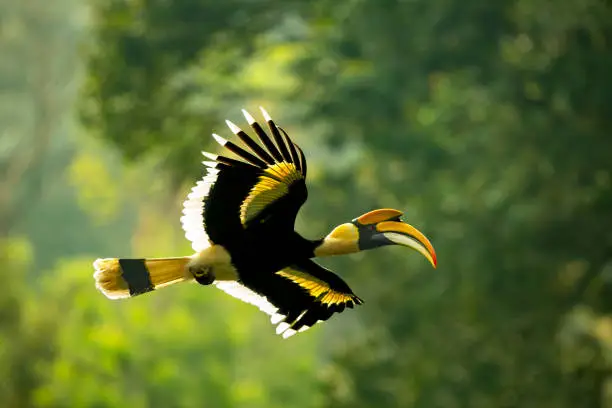
\includegraphics[width=\linewidth]{hornbill_image.png}
        \centering\scriptsize Great Hornbill in Flight
    \column{0.48\textwidth}
        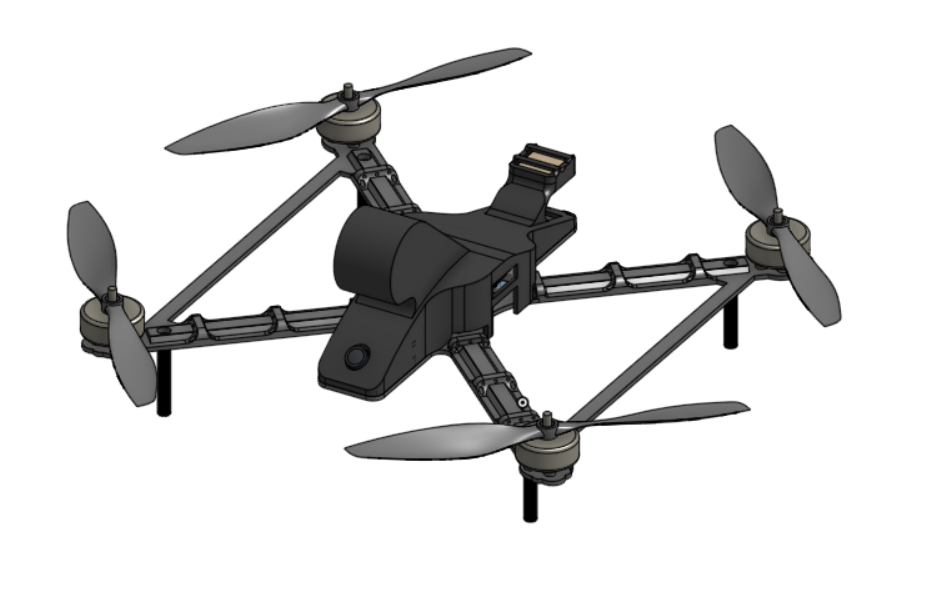
\includegraphics[width=\linewidth]{lulav_hornbill.png}
        \centering\scriptsize Lulav Hornbill Interceptor Drone
\end{columns}
\end{frame}

% --- CAPABILITIES ---
\begin{frame}{Performance Capabilities}
\begin{itemize}
    \item \textbf{Range \& Speed Options:}
    \begin{itemize}
        \item 2–5 km: 40–70 m/s
        \item 5–10 km: 30–60 m/s
        \item 10–20 km: 25–50 m/s
    \end{itemize}
    \item Day/Night interception capability
    \item Effective against Class 1–2 UAS
\end{itemize}
\end{frame}

% --- INTEGRATION ---
\begin{frame}{Integration Options}
\begin{itemize}
    \item Seamless integration with C2 systems
    \item Direct integration to radar or EO/IR sensors
    \item Full autonomy from detection to interception
\end{itemize}
\end{frame}

% --- SUMMARY ---
\begin{frame}{Mission Role}
\begin{block}{Rapid Response C-UAS}
    The Lulav Hornbill delivers unmatched agility and precision in neutralizing aerial threats.
    Inspired by the hornbill bird's aerial mastery, it combines high speed, autonomous control, and flexible integration.
\end{block}
\end{frame}

\end{document}
